%----------------------------------------------------------------
%
%  File    :  chapter1.tex
%
%  Authors :  Keith Andrews, IICM, TU Graz, Austria
%             Manuel Koschuch, FH Campus Wien, Austria
% 
%  Created :  22 Feb 96
% 
%  Changed :  24 March 2009
%  !TEX root = ./thesis.tex
%----------------------------------------------------------------

lol
\chapter{Einführung}
\label{chap:intro}
	Mobile App Development (MAD) und Software Engineering (SE) sollen den Entwicklungsprozess einer Software oder Mobilen Applikation insofern erleichtern, dass durch klar definierte Phasen der Entwicklungsprozess dokumentiert und verstanden wird \cite{Anthony2010}. Die Phasen bei SE beginnen mit der Analyse der Anforderungen an die zu entwickelnde Applikation. Durch gezielte Fragen und Diskussionen mit dem Kunden wird versucht ein erstes Bild von dem zu schaffen was nach Abschluss der Entwicklung der breiten Masse an Anwendern zur Verfügung gestellt werden soll. Anschließend wird es in der Design Phase spezifischer. In dieser Phase geht es nicht primär um das Aussehen und die Darstellung der unterschiedlichen User Interface (UI) Elemente sondern auch um die Spezifizierung der funktionalen und nicht funktionalen Anforderungen an die Anwendung \cite{Anthony2010}. Anschließend folgt die Phase der Implementierung gefolgt von einer Test Phase. Die Software geht anschließend an den Kunden bzw. an die Smartphone Anwender wenn es sich um eine Applikation handelt und wird in der Wartungsphase, im normal Fall einer kontinuierlichen Weiterentwicklung unterzogen. In der Wartungsphase geht es um die Behebung von \textit{Bugs} (Anwendungsfehler die einen Absturz der Applikation oder das Verwenden der Applikation erheblich erschweren), welche während der Testphase nicht gefunden wurden. 

	Diese Arbeit beschäftigt sich hauptsächlich mit den beiden ersten Phasen von SE und der Implementierung unter Xamarin.Forms als Cross-platform Framework. Xamarin und im besonderen Xamarin.Forms werden in Abschnitt \ref{chap:xamarin} genauer erläutert. Abschnitt \ref{chap:xamarin} bildet die Grundlage zu verstehen wie die Entwicklung mit einem CPF funktioniert und welche Überlegungen notwendig sind eine Applikation mit eben jenem Framework zu entwickeln.

	Jene Überlegungen die vor der Implementierung oder der ersten Programmierung von Funktionen der Applikation getroffen werden müssen, sind die Basis folgender Fragestellung mit welcher sich die Arbeit im zentralen beschäftigen wird:\vspace{1cm}

	\textit{Welche Einschränkungen ergeben sich durch Xamarin.Forms als Cross-platform Framework, im Vergleich zu Nativer Applikationsentwicklung unter Android und Cross-platform Entwicklung unter Xamarin.Native}?

\section{Motivation}
\label{sec:motivation}

	Smartphones haben heutzutage einen wichtigen Bestandteil des täglichen Lebens eingenommen. Der kurze Blick auf das Smartphone, auf dem Weg in die Schule oder in die Arbeit, sind Teil einer täglichen Routine geworden. Die Informationsbeschaffung ist durch mobiles Internet wie LTE (Long Term Evolution oder auch 4G) und immer schneller werdenderer Prozessoren in Smartphones einfacher denn je geworden. Doch nicht nur die Hardware der Anwender befindet sich in einem stetigen Prozess der Weiterentwicklung sondern auch die darauf laufende Software wie das Betriebssystem und diverse Applikationen. Apples iOS befindet sich derzeit in der Version 11.2.6 und wird bald Version 11.3.3 veröffentlichen. Im Vergleich dazu ist Android in Version 8.1.0 auf den aktuellsten Geräten bereits vorinstalliert. Apple begann mit seinem mobilen Betriebssystem iOS im Jahre 2005 und veröffentlichte 2007 iOS in der Version 1.0.x. Google begann 2008 seinen Start mit Android in der Version 1.0, auch bekannt als API 1. Seit der Einführung beider Betriebssysteme hat sich in den Jahren bis 2017 einiges getan. Gab es zu Beginn des Ersten Quartals 2009 noch folgende Vertreter:
	\begin{itemize}
		\setlength\itemsep{0em}
		\item Google - Android
		\item Apple - iOS
		\item Microsoft - Windows
		\item RIM - Blackberry
		\item Nokia - Symbian
	\end{itemize}

	Sind aktuell nur iOS und Android mit weltweiten Marktanteilen von 87,7\% für Android und 12,1\% für iOS übrig geblieben. Dies ist in Abbildung \ref{fig:mobile-os-marketshares} zu erkennen.

	Durch kontinuierliche Weiterentwicklung von Android und iOS erreichten diese eine immer größer werdende Beliebtheit wodurch andere Betriebssysteme weitgehend an Bedeutung verloren haben und schlussendlich keinen nennenswerten Anteil laut heutigen Statistiken besitzen.

	Jedoch sollte als Ausnahme die Firma RIM mit dem Betriebssystem BlackBerry OS erwähnt werden. Seit Blackberry OS 10 wurde es möglich Android Anwendungen ausführen zu können. Dies erzielte zwar nicht den erhofften Erfolg, war jedoch eine Besonderheit. Die Möglichkeit Anwendungen eines anderen Betriebssystems, wie zum Beispiel Android, installieren und auf die gleiche Art und Weise verwenden zu können ermöglichte es Anwendern, die Blackberry aufgrund seines außergewöhnlich Sicherheitsorientierten Betriebssystems verwendeten, das Beste aus beiden Welten zu vereinen.

	\newpage
	
	\begin{figure}[h!]
		\centering
		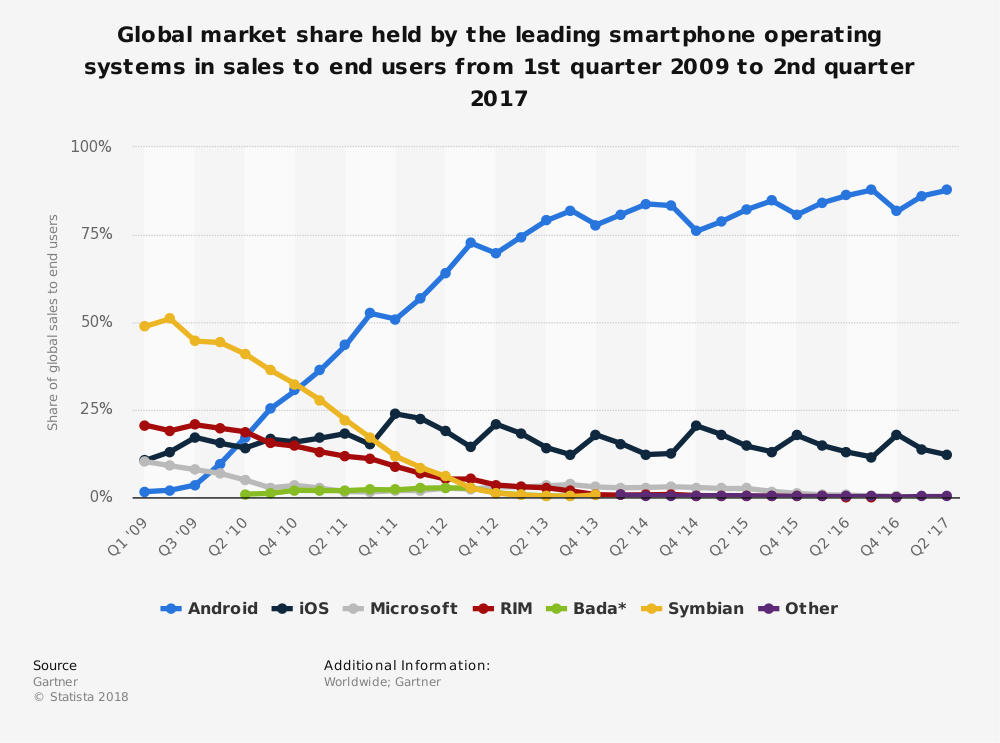
\includegraphics[width=1\textwidth]{images/statistic_id266136_global-mobile-os-market-share-2009-2017-by-quarter.png}
		\caption{Weltweiter Marktanteil an Mobilen Betriebssystemen von 2007 bis 2017 Stand Q1 2018 (Quelle: https://www.statista.com/statistics/266136/global-market-spare-held-by-smartphone-operating-systems/)}
		\label{fig:mobile-os-marketshares}
	\end{figure}
	Android ist aus heutiger Sicht das beliebteste Betriebssystem im weltweiten Vergleich. Doch warum finden sich in beiden App Stores, Google Play für Android und App Store für Apple, weit mehr als 2.000.000 Applikationen, wobei Android mit 3.361.843\footnote{https://de.statista.com/statistik/daten/studie/208599/umfrage/anzahl-der-apps-in-den-top-app-stores/} Anwendungen um mehr als 30\% mehr Applikationen als iOS zur Verfügung stellt. Diese Differenz scheint auf den Ersten Blick enorm, jedoch gilt es dabei folgenden Unterschied zu beachten. Applikationen können unter Android einfacher entwickelt und veröffentlicht werden. Apple zieht hier eine Grenze und gibt bestimmte Vorgaben vor und überprüft Apps genauer als Google. Weiters benötigt man einen Apple Developer Zugang der mit jährlichen Kosten verbunden ist.

	\newpage
	Die Motivation eine Cross-platform Applikation zu entwickeln ruht meist auf der Überlegung, warum man eine Applikation zwei Mal entwickeln muss, wenn sich eigentlich nur das Aussehen der Applikation verändert, nicht aber die grundlegenden Funktionalitäten \cite{Maximilian2017}. Als Beispiel dient die Facebook App die sowohl für Android als auch iOS mit React Native programmiert wurde. Demnach steht eine Vielzahl an CPF's der unterschiedlichsten Hersteller zur Verfügung.

	Folgende sind die populärsten \footnote{https://medium.com/@MasterOfCodeGlobal/best-10-android-frameworks-for-building-android-apps-d2d0ee48e464}:
	\begin{itemize}
		\setlength\itemsep{0em}
		\item Corona SDK - Spiel und Mobile App Development
		\item Xamarin
		\item Appcelerator Titanium
		\item React Native
		\item PhoneGap
		\item Iconic
		\item Sencha Touch
	\end{itemize}

	Alle CPF's bieten auf unterschiedlichste Art und Weise die Möglichkeit Applikationen auf Basis des \grqq Shared Codes\grqq, gemeinsame Funktionalitäten zusammenzufassen und nur einmal implementieren zu müssen. Der in der Integrierten Development Environment (IDE) eingebaute Compiler übernimmt die Aufgabe den Code entsprechend so zu kompilieren, damit dieser auf der Zielplattform nativ ausgeführt werden kann.

\newpage
\section{Related Work}
\label{sec:relatedwork}

Im Zuge der Literatur Recherche befassen sich einerseits, eine Vielzahl an Artikeln, Bachelor oder Master Arbeiten mit den Stärken und Schwächen von Cross-platform Frameworks, andererseits jedoch mit sehr spezifischen Themen der Applikationsentwicklung wie zum Beispiel Responsive UI Elements oder die Unterschiede wie ein Layout mit dem notwendigen Code dahinter interagiert und verknüpft wird. Dabei wird wiederum im speziellen auf die Kommunikation zwischen Layout und Code geachtet und analysiert.

Die Bücher \cite{book:Xamarin.Forms-Succinctly}, \cite{book:Xamarin.Forms-Essentials:} und \cite{book:Cross-platform-UI-Development-with-Xamarin.Forms} dienen als Grundlage um den Prozess der Implementierung einer Applikation mit der IDE zu verstehen und zu üben. Weiters gab es zwei Online Kurse um das in den Büchern erlernte Wissen praktisch umzusetzen.

Oleksandr Gridin widmet sich in seiner Bachelor Arbeit \cite{Oleksandr2015}, dem Xamarin Framework um dessen Stärken und Schwächen, anhand einer Android und Windows (Universal Windows Platform (UWP)) Applikation zu zeigen. Dabei wird sehr auf den Aufbau des Xamarin Frameworks, unter anderem auch Xamarin.Forms eingegangen. Im Zuge seiner Entwicklung ist es immer wieder zu Schwierigkeiten gekommen weil es keine oder nur wenige Komponenten gab um diverse Funktionalitäten umzusetzen.

In seiner Arbeit \cite{Armgren852125} \textit{Mobile Cross-platform development versus native development} widmet sich Armgren Marc, der  Performance von Xamarin als Cross-platform Framework in Bezug auf UI und Netzwerk Verkehr im Vergleich zu Nativer Applikations Entwicklung. Dabei wurden die Unterschiede zwischen Nativen iOS und Android und deren Cross-platform Pendant herangezogen. Die Evaluierung ergab das erst dann entschieden werden kann ob ein CPF verwendet werden soll wenn die Anforderungen klar definiert sind. Applikationen die eine Vielzahl an schwierigen Berechnungen durchführen müssen, wie zum Beispiel Spiele, profitierten von Nativen Code, da dieser performanter auf dem Zielbetriebssystem interpretiert und ausgeführt werden kann. In Bezug auf die Netzwerk Performance wurden keine Unterschiede festgestellt. 

Die Autoren V. Bhuttoo und K. Soman und R. K. Sungkur behandeln in dem Artikel \cite{8016193} die Stärken und Schwächen von Xamarin und stellen diese anderen bekannten Cross-platform Frameworks gegenüber. Dabei bedienten sie sich CPF's wie PhoneGap, verwendet HTML/CSS und Javascript um CP Apps zu entwickeln, und Titanium welches nur Javascript verwendet. Weiters beschäftigt sich dieser Artikel mit der Installation von CPF's und Komponenten des NuGET Paket Managers. Ihre Erkenntnisse zeigen das es überaus wichtig ist zu wissen welche Technologien Cross-platform Frameworks verwenden und wie man diese bestmöglich für eine CP App verwenden kann.

Die Arbeit von Ilke Soylemez \cite{Mukesh2016} erklärt wie die Entwicklung einer Cross-platform Applikation anhand eines Beispiels abläuft. Dabei wird vor allem auf essentielle Bausteine des Xamarin Frameworks eingegangen. Diese Bausteine sind unter anderem die Verwendung einer PCL (Portable Class Library) die, für die gemeinsame Geschäftslogik statt einer Shared Library, den Code der Cross-platform App implementiert. Weiters wird auf das MVVM (Model View View Model) Design Pattern von Xamarin eingegangen und wie dieses das Layout den notwendigen Code behind implementiert. Allerdings wird sich weitgehend mit Xamarin.Native befasst wobei das MVVM Design Pattern sowohl bei Xamarin.Native als auch bei Xamarin.Forms zum Einsatz kommt.

In meiner vorigen Arbeit zum Thema Cross-platform Development \cite{Maximilian2017} wurde die Entwicklung einer Cross-platform Applikation auf Basis einer Nativen Applikation betrachtet. Dabei ging es vorrangig um Xamarin als CPF und welche Unterschiede oder Schwierigkeiten bei der Entwicklung einer Cross-platform App im Vergleich zu Nativer Applikationsentwicklung auftreten. Dabei wurde eine in JAVA unter Android Studio entwickelte Applikation erneut spezifiziert und unter Xamarin.Native für Android und iOS implementiert. Im Zuge der erneuten Anforderungsanalyse und Design Phase konnten während der Implementierung einige Zeilen an Code eingespart werden, da Xamarin Komponenten beispielsweise für eine Kommunikation mit einer SQL Datenbank zur Verfügung stellt in die PCL Klasse ausgelagert werden wodurch diese Kommunikation mit einem Server nur einmal implementiert werden musste. Beide Applikationen konnten durch aufrufen der Funktionen den selben Code ausführen. Allerdings verlangte Xamarin.Native das Design der App zweimal zu Entwickeln, was einen enormen Programmieraufwand verlangte.
